\documentclass[main.tex]{subfiles}
\begin{document}

\chapter{The Neyman--Pearson Lemma and Most Powerful Tests}\label{ch:neyman-pearson}\chaptermark{The Neyman--Pearson Lemma}

Estimation answers the question ``what is $\theta$?''; hypothesis testing\index{hypothesis test@hypothesis test} answers the question ``are the data consistent with a particular claim about $\theta$?''. The contribution of Neyman and Pearson in 1933 \cite{neyman-pearson33} was to set up the testing problem as an optimisation problem: bound the probability of a type I\index{type i and type ii errors@type I and type II errors} error at a prespecified level $\alpha$ and, subject to this constraint, minimise the type II error (maximise the power). For two simple hypotheses the solution is surprisingly simple: reject $H_0$ where the likelihood ratio\index{likelihood ratio@likelihood ratio} is large. This chapter lays the foundation for the next three (UMP\index{uniformly most powerful ump test@uniformly most powerful (UMP) test} tests, likelihood ratio tests\index{likelihood ratio test lrt@likelihood ratio test (LRT)}, confidence intervals).

\section{Definitions}

\begin{definition}[Hypotheses]
Let $\Theta=\Theta_0\cup\Theta_1$ be a disjoint decomposition. $H_0:\theta\in\Theta_0$ is the \emph{null hypothesis\index{null hypothesis@null hypothesis}} and $H_1:\theta\in\Theta_1$ the \emph{alternative hypothesis}. If $\Theta_j$ consists of a single point the hypothesis is \emph{simple}, otherwise it is \emph{composite}.
\end{definition}

\begin{definition}[Test Function]
A \emph{(randomised) test} is a measurable function $\phi:\mathcal X^n\to[0,1]$: when $\x$ is observed, $H_0$ is rejected with probability $\phi(\x)$. If $\phi\in\{0,1\}$ the test is \emph{non-randomised} and $\mathcal R=\{\x:\phi(\x)=1\}$ is its \emph{rejection region}.
\end{definition}

\begin{definition}[Error Types and the Power Function]
\[
\beta_\phi(\theta)=\E_\theta[\phi(\X)]\qquad(\text{power function}).
\]
For $\theta\in\Theta_0$, $\beta_\phi(\theta)$ is the probability of a \emph{type I\index{type i and type ii errors@type I and type II errors} error}; for $\theta\in\Theta_1$, $1-\beta_\phi(\theta)$ is the probability of a \emph{type II error} and $\beta_\phi(\theta)$ is the \emph{power} of the test at $\theta$.
\end{definition}

\begin{definition}[Level and Size]
$\sup_{\theta\in\Theta_0}\beta_\phi(\theta)$ is called the \emph{size} of the test. A test with size $\le\alpha$ is called a \emph{level-$\alpha$} test.
\end{definition}

\begin{definition}[Most Powerful (MP) Test]
For simple hypotheses $H_0:\theta=\theta_0$, $H_1:\theta=\theta_1$, a level-$\alpha$ test $\phi^*$ is \emph{most powerful} (MP) if $\beta_{\phi^*}(\theta_1)\ge\beta_\phi(\theta_1)$ for every level-$\alpha$ test $\phi$.
\end{definition}

\begin{definition}[$p$-Value]\label{def:p-degeri}
Let $\{\mathcal R_\alpha\}_{\alpha\in(0,1)}$ be nested rejection regions satisfying $\alpha'<\alpha\implies\mathcal R_{\alpha'}\subseteq\mathcal R_\alpha$. The value $p(\x)=\inf\{\alpha:\x\in\mathcal R_\alpha\}$ is called the \emph{$p$-value}: the smallest level at which $H_0$ can be rejected with the observed data. For tests of the form ``reject for large $T$'', $p(\x)=\sup_{\theta\in\Theta_0}\P_\theta(T(\X)\ge T(\x))$.
\end{definition}

\section{The Neyman--Pearson Lemma}

\begin{theorem}[Neyman--Pearson Lemma \cite{neyman-pearson33}]\label{thm:neyman-pearson}\index{neyman pearson lemma@Neyman--Pearson lemma}
Let $H_0: \theta = \theta_0$, $H_1: \theta = \theta_1$ and $f_j(\x)=L(\theta_j;\x)$.
\begin{enumerate}
  \item \textbf{(Sufficiency)} If for some $k\ge0$ and $\gamma\in[0,1]$
  \[
  \phi^*(\x)=\begin{cases}1, & f_1(\x)>kf_0(\x)\\ \gamma, & f_1(\x)=kf_0(\x)\\ 0, & f_1(\x)<kf_0(\x)\end{cases}\qquad\text{and}\qquad\E_{\theta_0}[\phi^*(\X)]=\alpha,
  \]
  then $\phi^*$ is a most powerful (MP) level-$\alpha$ test.
  \item \textbf{(Existence)} For every $\alpha\in(0,1)$ there is a test of this form with size exactly $\alpha$.
  \item \textbf{(Necessity)} If $\phi$ is any MP level-$\alpha$ test, then $\phi=\phi^*$ a.e.\ on the set $\{f_1\ne kf_0\}$.
\end{enumerate}
Randomisation is needed only for discrete distributions; for continuous distributions $\P_{\theta_0}(f_1=kf_0)=0$ and the test reduces to $\phi^*(\x) = \I\{L(\theta_1)/L(\theta_0) > k\}$.
\end{theorem}
\begin{proof}
(1) Let $\phi$ be any level-$\alpha$ test. For every $\x$,
\[
\big(\phi^*(\x)-\phi(\x)\big)\big(f_1(\x)-kf_0(\x)\big)\ge0,
\]
because when $f_1>kf_0$, $\phi^*=1\ge\phi$; when $f_1<kf_0$, $\phi^*=0\le\phi$; and in the case of equality the second factor is zero. Integrating,
\[
\beta_{\phi^*}(\theta_1)-\beta_\phi(\theta_1)\ge k\big(\beta_{\phi^*}(\theta_0)-\beta_\phi(\theta_0)\big)=k\big(\alpha-\beta_\phi(\theta_0)\big)\ge0 .
\]
(2) Let $R(\x)=f_1(\x)/f_0(\x)$ (on $f_0>0$) and $a(c)=\P_{\theta_0}(R>c)$. $a$ is a non-increasing, right-continuous function of $c$ (the complement of a CDF). Choosing $k=\inf\{c: a(c)\le\alpha\}$ gives $a(k)\le\alpha\le a(k^-)=\P_{\theta_0}(R\ge k)$. If $\P_{\theta_0}(R=k)>0$ take $\gamma=\frac{\alpha-a(k)}{\P_{\theta_0}(R=k)}\in[0,1]$, otherwise $\gamma=0$; the size is then exactly $\alpha$.
(3) If $\phi$ is MP, the inequality in (1) must be an equality; a non-negative integrand with zero integral is zero a.e., i.e.\ $\phi=\phi^*$ wherever $f_1\ne kf_0$.
\end{proof}

\begin{corollary}[An MP Test Is Unbiased]\label{cor:mp-yansiz}
If $\phi^*$ is an MP test\index{most powerful mp test@most powerful (MP) test} of level $\alpha\in(0,1)$, then $\beta_{\phi^*}(\theta_1)\ge\alpha$; if $f_0\neq f_1$, the inequality is strict.
\end{corollary}
\begin{proof}
The test $\phi\equiv\alpha$, which does not use the data at all, has level $\alpha$ and power $\alpha$; the MP test must be at least as powerful.
\end{proof}

\begin{corollary}[Expression via a Sufficient Statistic]\label{cor:np-yeterli}
If $T$ is sufficient and $g(t;\theta_j)$ is the factor in the factorisation\index{factorisation theorem@factorisation theorem}, then the MP test has the form $g(T;\theta_1)/g(T;\theta_0)>k$; that is, it depends only on $T$.
\end{corollary}
\begin{proof}
By factorisation, $f(\x;\theta_j)=g(T(\x);\theta_j)h(\x)$. For every $\x$ with $h(\x)>0$,
$\frac{f(\x;\theta_1)}{f(\x;\theta_0)}=\frac{g(T(\x);\theta_1)}{g(T(\x);\theta_0)}$; the points with $h(\x)=0$ have probability zero under both hypotheses, and how the test is defined there affects neither its level nor its power. Apply Theorem~\ref{thm:neyman-pearson}.
\end{proof}

\begin{theorem}[Distribution of the $p$-Value]\label{thm:p-uniform}
If the distribution of $T$ under (simple) $H_0$ is continuous and the test has the form ``reject for large $T$'', then $p(\X)=1-F_0(T(\X))\sim\text{Uniform}(0,1)$ under $H_0$. For discrete $T$, $\P_{\theta_0}(p(\X)\le u)\le u$ (stochastically larger than uniform).
\end{theorem}
\begin{proof}
By the probability integral transform\index{probability integral transform@probability integral transform} (Theorem~\ref{thm:pit}), $F_0(T)\sim\text{Uniform}(0,1)$, and therefore so is $1-F_0(T)$.
\end{proof}

\section{Worked Examples}

\begin{example}[Normal Mean: MP Test and the Power Formula]\label{ex:normal-mp}
$X_i\iid\Normal(\mu,\sigma^2)$ with $\sigma$ known; $H_0:\mu=\mu_0$, $H_1:\mu=\mu_1>\mu_0$. The likelihood ratio\index{likelihood ratio@likelihood ratio}
\[
\frac{L(\mu_1)}{L(\mu_0)}=\exp\Big\{\frac{\mu_1-\mu_0}{\sigma^2}\sum x_i-\frac{n(\mu_1^2-\mu_0^2)}{2\sigma^2}\Big\}
\]
is an increasing function of $\bar x$. Hence the MP test\index{most powerful mp test@most powerful (MP) test} has the form $\bar X>c$, and $\P_{\mu_0}(\bar X>c)=\alpha$ gives $c=\mu_0+z_\alpha\sigma/\sqrt n$. Power:
\[
\beta(\mu_1)=\P_{\mu_1}(\bar X>c)=1-\Phi\Big(z_\alpha-\frac{\sqrt n(\mu_1-\mu_0)}{\sigma}\Big).
\]
With $\mu_0=0$, $\mu_1=1$, $\sigma=2$, $n=16$, $\alpha=0.05$: $c=1.645\cdot0.5=0.822$ and $\beta=1-\Phi(1.645-2)=\Phi(0.355)\approx0.639$.

Note: the critical value $c$ \emph{does not depend on $\mu_1$}. This observation is the key to the UMP\index{uniformly most powerful ump test@uniformly most powerful (UMP) test} tests of Chapter~\ref{ch:karlin-rubin}.
\end{example}

\begin{example}[Sample Size Calculation]\label{ex:orneklem-guc}
In the same problem, the $n$ required for a level-$\alpha$ test with power $1-\beta$ is
\[
z_\alpha-\frac{\sqrt n\,\Delta}{\sigma}=-z_\beta\implies n=\Big(\frac{(z_\alpha+z_\beta)\sigma}{\Delta}\Big)^2,\qquad\Delta=\mu_1-\mu_0 .
\]
For $\sigma=2$, $\Delta=1$, $\alpha=0.05$ and power $0.80$ ($z_{0.20}=0.842$), $n=(2.487\cdot2)^2\approx24.7$, i.e.\ $n=25$.
\end{example}

\begin{example}[Poisson: A Randomised MP Test]\label{ex:poisson-rastgele}
$X_1,\dots,X_{10}\iid\text{Poisson}(\lambda)$, $H_0:\lambda=1$, $H_1:\lambda=2$, $\alpha=0.05$. $T=\sum X_i$ is sufficient and the likelihood ratio $(2/1)^Te^{-10}$ is increasing in $T$. Under $H_0$, $T\sim\text{Poisson}(10)$. Since $\P_0(T\ge16)\approx0.0487<0.05<\P_0(T\ge15)\approx0.0835$ (values verified with the code below), no non-randomised test\index{randomised test@randomised test} can have size exactly $0.05$. The MP test is
\[
\phi^*(T)=\begin{cases}1, & T\ge16\\ \gamma, & T=15\\ 0,& T\le14\end{cases},\qquad\gamma=\frac{0.05-\P_0(T\ge16)}{\P_0(T=15)}.
\]
\end{example}

\begin{example}[Normal Variance]
$X_i\iid\Normal(0,\sigma^2)$, $H_0:\sigma^2=\sigma_0^2$, $H_1:\sigma^2=\sigma_1^2>\sigma_0^2$. The likelihood ratio is increasing in $\sum x_i^2$; since $\sum X_i^2/\sigma_0^2\sim\chi^2_n$ under $H_0$, the MP test rejects when $\sum X_i^2>\sigma_0^2\chi^2_{n,\alpha}$.
\end{example}

\section{Computational Applications}

\subsection{Power of the Test for a Normal Mean}

\pycode{code/ch13/c13_1_power_normal_mean_test.py}
\begin{lstlisting}[style=output]
Critical value c = 0.8224
Type I error (MC): 0.0497  (target 0.05)
Neyman-Pearson power: 0.6397
Analytic power       : 0.6388
Required n for power 0.80 = 24.73
\end{lstlisting}

\subsection{A Randomised Poisson Test}

\pycode{code/ch13/c13_2_randomised_poisson_test.py}
\begin{lstlisting}[style=output]
Reject: T > 15 ; if T = 15 reject with probability gamma = 0.0363
P0(T >= 16) = 0.0487 | P0(T >= 15) = 0.0835
Size = 0.0500
Power (randomised)        = 0.8454
Power (T > 15, conservative) = 0.8435
Power (simulation)        = 0.8452
\end{lstlisting}

\subsection{Power Curves and the Distribution of $p$-Values}

\pycode{code/ch13/c13_3_power_curves_pvalue_distribution.py}
\begin{lstlisting}[style=output]
mu=0.0: P(p <= 0.05) = 0.0503
mu=0.5: P(p <= 0.05) = 0.2606
\end{lstlisting}

\begin{figure}[h]
\centering
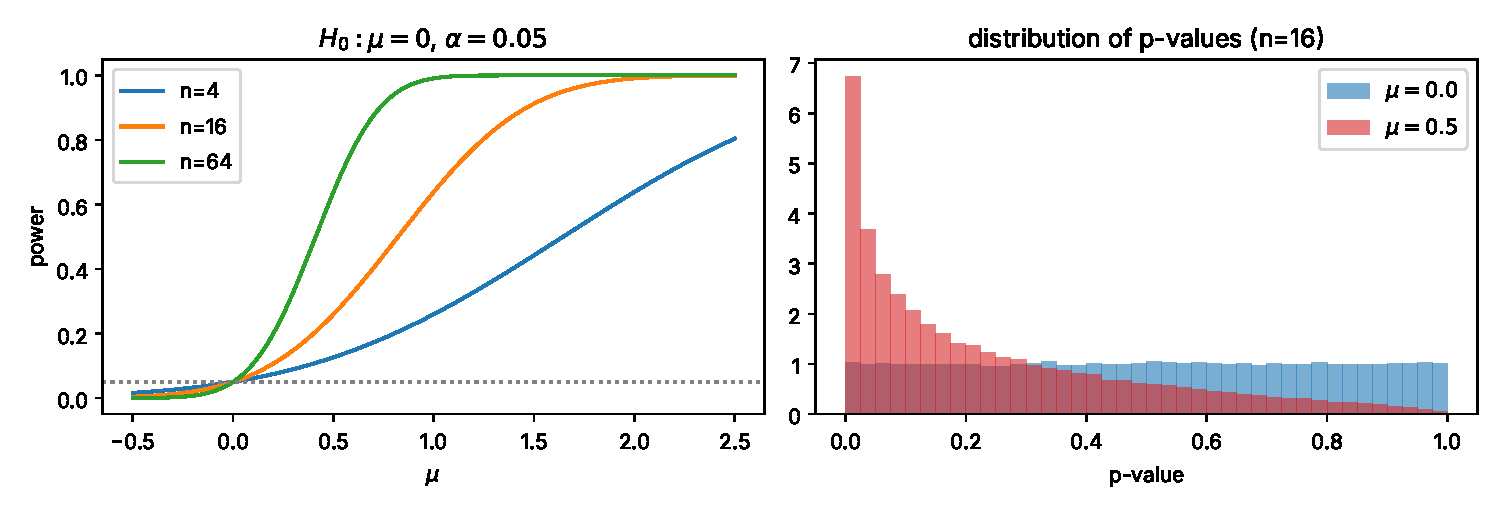
\includegraphics[width=\textwidth]{figures/guc_pdeger.pdf}
\caption{Left: power functions of the one-sided $z$-test; all curves pass through $\alpha$ at $\mu=0$ and become steeper as $n$ grows. Right: when $H_0$ is true the $p$-values are uniformly distributed (Theorem~\ref{thm:p-uniform}); under $H_1$ they pile up near zero.}
\end{figure}

\section{Comments and Notes}

\begin{remark}[An Asymmetric Approach]
The Neyman--Pearson\index{neyman pearson lemma@Neyman--Pearson lemma} framework does not treat $H_0$ and $H_1$ symmetrically: the type I\index{type i and type ii errors@type I and type II errors} error is kept under control, while the type II error is only minimised. Therefore ``$H_0$ could not be rejected'' does not mean ``$H_0$ is true''; a low-power test frequently fails to reject $H_0$. This is why power analysis is an integral part of experimental design.
\end{remark}

\begin{remark}[Randomisation in Practice]
Randomised tests\index{randomised test@randomised test} are needed in theory (for the existence of an MP test\index{most powerful mp test@most powerful (MP) test}), but they are rarely used in practice, because the same data can lead to different decisions. Practitioners report either the conservative test ($\gamma=0$) or the $p$-value; the ``mid-$p$'' value $\P(T>t)+\frac12\P(T=t)$ is a compromise.
\end{remark}

\begin{remark}[What Does a $p$-Value Not Measure?]
The $p$-value is \emph{not} the probability that $H_0$ is true; it is the probability, when $H_0$ is true, of obtaining a result at least as extreme as the one observed. Nor does it measure effect size: for very large $n$, even negligibly small differences produce very small $p$-values. The 2016 statement of the American Statistical Association \cite{wasserstein16} discusses these misinterpretations in detail. The relationship between $p$-values and posterior probabilities is taken up in Chapter~\ref{ch:bayes}.
\end{remark}

% --- CHAPTER SUMMARY ---
\section{Chapter Summary}
\begin{summary}
\begin{itemize}
  \item A test is a decision rule. The probability of a type I error is bounded by the level, and the power is maximised subject to this constraint.
  \item The Neyman--Pearson lemma (Theorem~\ref{thm:neyman-pearson}): for simple hypotheses the most powerful test is the likelihood ratio test. For discrete distributions, randomisation may be needed to attain the level exactly.
  \item An MP test is unbiased (Corollary~\ref{cor:mp-yansiz}) and depends only on a sufficient statistic (Corollary~\ref{cor:np-yeterli}).
  \item The $p$-value (Definition~\ref{def:p-degeri}) is the probability under $H_0$ of a result at least as extreme as the one observed; for a continuous test statistic it is uniformly distributed under $H_0$ (Theorem~\ref{thm:p-uniform}). The $p$-value is not the probability that $H_0$ is true, and it does not measure effect size.
\end{itemize}
\end{summary}
% --- END OF CHAPTER SUMMARY ---

\paragraph{Further reading.} \cite[Chapter~8]{casella}, \cite[Chapter~3]{lehmann-romano}, \cite[Chapter~10]{wasserman}.

\section{Exercises}

\begin{exercise}\label{exr:13-1}
$X\sim\text{Uniform}(0,\theta)$, a single observation. Find the MP level-$\alpha$ test of $H_0:\theta=1$ against $H_1:\theta=2$. Show that the likelihood ratio (on the region where $f_0>0$ or $f_1>0$) takes only two values ($1/2$ and $\infty$) and that the MP test is not unique.
\hfill\hyperref[coz:13-1]{\footnotesize$\rightarrow$\,Solution}
\end{exercise}

\begin{exercise}\label{exr:13-2}
$X_i\iid\text{Bernoulli}(p)$, $n=20$, $H_0:p=0.5$, $H_1:p=0.7$. Construct the randomised MP test at level $\alpha=0.05$ and compute its power.
\hfill\hyperref[coz:13-2]{\footnotesize$\rightarrow$\,Solution}
\end{exercise}

\begin{exercise}\label{exr:13-3}
$H_0:X\sim\Normal(0,1)$, $H_1:X\sim\text{Cauchy}(0,1)$ (a single observation). Show that the rejection region of the MP test has the form $\{|x|>c\}$ and compute the power for $\alpha=0.05$. (Is the likelihood ratio a monotone function of $x^2$?)
\hfill\hyperref[coz:13-3]{\footnotesize$\rightarrow$\,Solution}
\end{exercise}

\begin{exercise}\label{exr:13-4}
Using Theorem~\ref{thm:p-uniform}, show that for the $p$-values of $m$ independent tests the Bonferroni correction (performing each test at level $\alpha/m$) bounds the family-wise error rate by $\alpha$ (Chapter~\ref{ch:olasilik-uzaylari}, Boole's inequality).
\hfill\hyperref[coz:13-4]{\footnotesize$\rightarrow$\,Solution}
\end{exercise}

\end{document}
